\documentclass{article}

\usepackage{enumerate}
\usepackage{amsmath}
\usepackage[letterpaper, margin=1in]{geometry}
\usepackage{tikz}
\usetikzlibrary{shapes,shapes.arrows,positioning}

\begin{document}	
	\begin{enumerate}[\textbf{{1}.1}]
		\item \quad
		\begin{itemize}
			\item [9.]
			\item [14.]
			\item [22.]
		\end{itemize}
		
		\item \quad
		\begin{itemize}
			\item [4.]
			\item [6.] \quad
			\begin{enumerate}[(a)]
				\item 
			\end{enumerate}
		\end{itemize}
		
		\item \quad
		\begin{itemize}
			\item [3.] \quad
			\begin{itemize}
				\item [(c)]
				\item [(d)]
			\end{itemize}
			
			\item [5.] \quad
			\begin{itemize}
				\item [(a)]
				\item [(c)]
			\end{itemize}
			
			\item [8.] \quad
			\begin{enumerate}[(a)]
				\item
				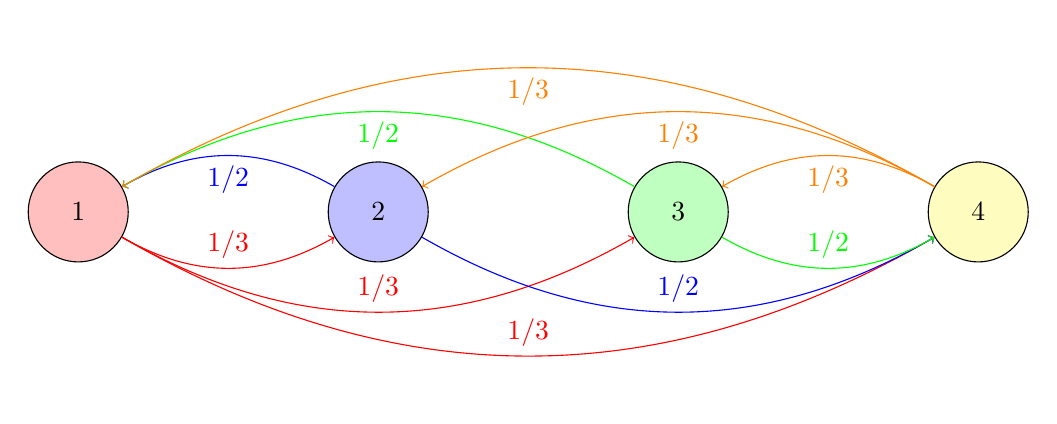
\begin{tikzpicture}[->, node distance=1.5in, baseline={(current bounding box.north)}]
					\centering
					\node [circle, draw, minimum size=0.5in, fill=red!25] (one) {1};
					\node [circle, draw, minimum size=0.5in, fill=blue!25] (two) [right of=one] {2};
					\node [circle, draw, minimum size=0.5in, fill=green!25] (three) [right of=two] {3};
					\node [circle, draw, minimum size=0.5in, fill=yellow!25] (four) [right of=three] {4};
					\path (one) edge [red] [bend right] node [above] {$1/3$} (two);
					\path (one) edge [red] [bend right] node [above] {$1/3$} (four);
					\path (one) edge [red] [bend right] node [above] {$1/3$} (three);
					\path (two) edge [blue] [bend right] node [below] {$1/2$} (one);
					\path (two) edge [blue] [bend right] node [above] {$1/2$} (four);
					\path (three) edge [green] [bend right] node [below] {$1/2$} (one);
					\path (three) edge [green] [bend right] node [above] {$1/2$} (four);
					\path (four) edge [orange] [bend right] node [below] {$1/3$} (one);
					\path (four) edge [orange] [bend right] node [below] {$1/3$} (two);
					\path (four) edge [orange] [bend right] node [below] {$1/3$} (three);
				\end{tikzpicture}
				\item
			\end{enumerate}
		\end{itemize}
	\end{enumerate}
\end{document}